\documentclass{article}
\usepackage{epsfig}
\usepackage{latexsym}
\usepackage{amsmath}
\usepackage{fullpage}
% This is to print nomenclature
\usepackage{makeidx}
\makeindex
\usepackage{nomencl}
\makenomenclature
% Macro of list of symbols
%\def\listofsymbols{\input{symbols} \clearpage}
%\def\addsymbol #1: #2#3{$#1$ \> \parbox{5in}{#2 \dotfill \pageref{#3}}\\}
%\def\newnot#1{\label{#1}}


%\renewcommand{\thefootnote}

\nomenclature{$\mathbf{I}$}{identity matrix}%
\nomenclature{$\delta$}{Kronecker delta}%
\nomenclature{$\Pi$}{volume of the complete domain}%
\nomenclature{$\mathbf{R}$}{residual}%
\nomenclature{$\Psi$}{weight of the residual}%
\nomenclature{$\mathbf{\Sigma(x)}$}{stress at position $\mathbf{x}$}%
\nomenclature{$\mathbf{\sigma_c(x)}$}{meaured stress at position $\mathbf{x_c}$}%
\nomenclature{$s^{ij}_I$}{ij component of stress at the node I}%
\nomenclature{$\mathbf{s}_I$}{elemental stress vector at the global node I in the mesh}%
\nomenclature{$\mathbf{s}$}{stress vector containing all the nodes of an element}%
\nomenclature{$\mathbf{S}_I$}{global stress vector at the global node I in the mesh}%
\nomenclature{$N_I$}{shape functions of node I}%
\nomenclature{$N^s_I$}{surface shape functions of node I}%
\nomenclature{$\mathbf{N}$}{matrix formed by the shape functions for the nodes of an element $\forall$ dof}%
\nomenclature{$\mathbf{N^s}$}{matrix formed by the shape functions for the surface nodes of an element $\forall$ dof}%
\nomenclature{$\mathbf{\overline{N}}$}{vectorized form of shape functions for an element}%
\nomenclature{$\mathbf{\overline{N}^s}$}{vectorized form of surface shape functions for an element}%
\nomenclature{$\mathbf{\overline{0}}$}{zero vector}%
\nomenclature{$n$}{number of nodes per element}%
\nomenclature{$ns$}{number of surface nodes per element}%
\nomenclature{$V$}{volume of an element}%
\nomenclature{$A$}{area of an element}%
\nomenclature{$\mathbf{M^{el}}$}{elemental premultiplier of nodal stresses}%
\nomenclature{$\mathbf{F^{el}}$}{elemental measured stress vector}%
\nomenclature{$\mathbf{F}_I$}{global measured stress vector}%
\nomenclature{$\mathbf{M}_I$}{global (assembled) premultiplier of nodal stresses}%
\nomenclature{$\mathbf{B}$}{a special matrix formed by the derivative of shape functions}%
\nomenclature{$\mathbf{C^{el}}$ }{elemental equilibrium constraint matrix}%
\nomenclature{$\mathbf{C}_I$}{global equilibrium constraint matrix}%
\nomenclature{$\mathbf{t(x)}$}{surface traction vector}%
\nomenclature{$\mathbf{s^s}$}{stress vector containing all the nodes of the surface of an element}%
\nomenclature{$\mathbf{T^{el}}$ }{elemental traction-free surface constraint matrix}%
\nomenclature{$\mathbf{T}_I$}{global traction-free surface constraint matrix}%
\nomenclature{$\mathbf{P}$}{mapping to get tractions from the stress components}%
\nomenclature{$\mathbf{r}$}{surface normal}%
\nomenclature{$\mathbf{G}$}{mapping to get in-plane surface tractions from surface tractions}%
\nomenclature{$\mathbf{D^{el}}$}{elemental symmetry surface constraint matrix}%
\nomenclature{$\mathbf{D}_I$}{global symmetry surface constraint matrix}%
\nomenclature{$\mathbf{J}$}{mapping that gives in-plane tractions from the stress components}%
\nomenclature{$\mathbf{K}$}{finite element constraints}%
\nomenclature{$\mathbf{Q}$}{mapping between orientation averaged stress and nodal stress vector}%
\nomenclature{$\mathbf{L}$}{mapping between harmonic coefficients and orientation averaged stress}%
\nomenclature{$\mathbf{A}$}{mapping between lattice strains and harmonic coefficients}%
\nomenclature{$\mathbf{\epsilon}$}{lattice strains obtain by diffraction measurements}%
\nomenclature{$\mathbf{p}$}{monomial with a linear basis}%
\nomenclature{$\mathbf{a(x)}$}{coefficients of monomial used in MLS method}%
\nomenclature{$\mathbf{\sigma_c(x)}$}{interpolated value of measured stress at any position $\mathbf{x}$}%
\nomenclature{$x, y, z$}{coordinate positions}%
\nomenclature{$ndv$}{number of diffraction measurement locations}%
\nomenclature{$w$}{weight used in MLS method}%
\nomenclature{$J$}{square norm of the residual used in MLS method}%
\nomenclature{$\mathbf{Y}$}{a mapping used to construct interpolation function used in MLS method}%
\nomenclature{$\mathbf{Z}$}{another mapping used to construct interpolation function used in MLS method}%
\nomenclature{$q$}{distance from the position of measurement used in MLS method}%
\nomenclature{$\rho$}{constant radius of spheres used in MLS method}%
\nomenclature{$\kappa$}{scaling constant for the ellipsoids}%
\nomenclature{$\lambda$}{penalty factor for the equilibrium constraint}%
\nomenclature{$\beta$}{penalty factor for the traction-free constraint}%
\nomenclature{$\alpha$}{penalty factor for the symmetry-surface constraint}%
\nomenclature{$\xi, \eta, \zeta$}{natural (mapped) coordinates of elements}%
\begin{document}
\date{}



\title{3d residual stress project}
\maketitle





%\newpage
%\chapter*{List of Symbols\hfill} \addcontentsline{toc}{chapter}{List of Symbols}
%\listofsymbols
\addcontentsline{toc}{chapter}{Nomenclature}
\printnomenclature

The object of this analysis is to find the stress distribution in a body (i.e. machine component, sample after a forming process) using lattice strain measurements. That is called residual stress but it should not be confused with the residual used in the analysis.

Residual refers to the difference between the measured orientation averaged stresses that are measured from diffraction experiments and the macroscopic stress distribution which are obtained from the nodal values of stress. Body under interest is discretized with finite elements. The objective is to find the nodal values of stresses that minimize the residual\footnote{Bold fonts are used indicate matrices and vectors.}, $\mathbf{R}$, weakly (in an integral form) as in eq. \eqref{eqres}.

In eq. \eqref{eqres}, the difference between the macroscopic stress, $\mathbf{\Sigma(x)}$, at position $\mathbf{x}$, and the stress measured, $\mathbf{\sigma_c}$, at position at $\mathbf{x_c}$, is minimized over the domain $\Pi$. $\Psi$ is the weight of the residual. The measured stress, $\mathbf{\sigma_c}$, is an orientation averaged quantity and it is obtained from the lattice strain measurements (More details are discussed in section \ref{sectINV}). 
\begin{equation}
\mathbf{R} \,=\, \int_\Pi \Psi \, [\mathbf{\Sigma(x)} \, -\delta(\mathbf{x}-\mathbf{x_c}) \mathbf{\sigma_c}] \,d\Pi
\label{eqres}
\end{equation}

Later on, several other physical constraints acting on the body, $\Pi$, (i.e. equilibrium, traction free surfaces) will be introduced to the residual. 


%Diffraction measurements tells the amount of lattice strains for a grain orientation. Lattice strains can be converted into stresses using single crystal elasticity matrix. Note, the elastic anisotropy is included to the analysis at this point.


%There may be two different kinds of experimental limitations. \textbf{i.} Practically, stress can be measured at only certain regions in reasonable measurement times due to geometrical limitations. \textbf{ii.} Diffraction measurements may not cover all of the individual grains in a diffraction volume that comprise of many number of grains. Hence, using the residual analysis by enforcing physical constraints, we want to obtain the complete stress distribution in the body from the measurements.

\section{residual}
Residual is indicated with $\mathbf{R}$ in eq. \eqref{eqres} which comprises of two main integrals of \ref{sect1} macroscopic stress (to be calculated from the nodal stresses) and, \ref{sect2} measured stress vector.
 
\subsection{macroscopic stress}\label{sect1}
Eq. \eqref{intstress} shows an example use of interpolation functions to find the magnitude of $zz$ component of stress, $\Sigma(x)^{zz}$, in an element at position $\mathbf{x}$ using the nodal values of stress $s^{zz}_I$ and the shape function of that element $N_I(\mathbf{x})$. The subscript $I$ refers to the node number of that element. Shape functions of different elements are shown in appendix A.
\begin{equation}
\Sigma^{zz}(x) \,=\, \sum_I \, N_I(\mathbf{x}) \, s^{zz}_I
\label{intstress}
\end{equation}

For a general case, stress has 6 degrees of freedom (dof) that are independent of each other. Hence, to interpolate all 6 components of stress, we write eq. \eqref{intstress} for each stress component as a matrix equation, \eqref{eqis}. 
\begin{equation}
\mathbf{\Sigma(x)} \,=\, \, \mathbf{N(\mathbf{x})} \, \mathbf{s}
\label{eqis}
\end{equation}

$\mathbf{s}$ is the vector that consists of nodal stress vectors, $\mathbf{s}_I$, as shown in eq. \eqref{eqs} where $n$ number of nodes per element. The superscript $T$ is used to indicate transpose.
\begin{equation}
\mathbf{s}\,=\, \, \left[\; \mathbf{s}_1\; \mathbf{s}_2 \; \cdots\; \mathbf{s}_n\; \right]^T
\label{eqs}
\end{equation}



$\mathbf{s}_I$ is the vectorized form of stress at each node $I$ as in eq. \eqref{eq1}.
\begin{equation}
\mathbf{s}_I = \left[{
\begin{array}{cc}
	s^{xx}_I\\
	s^{yy}_I\\
	s^{zz}_I\\
	s^{xy}_I\\
	s^{xz}_I\\
	s^{yz}_I\\
\end{array}} \right]
\label{eq1}
\end{equation}


In eq. \eqref{eq3}, $\mathbf{N}$ is a matrix formed by the shape functions and by the zero vectors for 6 dof calculated at any position $\mathbf{x}$. Positions are not indicated anymore for simplicity. 
\begin{equation}
\mathbf{N} = \left[{ \begin{array}{cccccc}
		\mathbf{\overline{N}} & \mathbf{\overline{0}} & \mathbf{\overline{0}} & \mathbf{\overline{0}} & \mathbf{\overline{0}} & \mathbf{\overline{0}} \\
		\mathbf{\overline{0}} & \mathbf{\overline{N}} & \mathbf{\overline{0}} & \mathbf{\overline{0}} & \mathbf{\overline{0}} & \mathbf{\overline{0}} \\
		\mathbf{\overline{0}} & \mathbf{\overline{0}} & \mathbf{\overline{N}} & \mathbf{\overline{0}} & \mathbf{\overline{0}} & \mathbf{\overline{0}} \\
		\mathbf{\overline{0}} & \mathbf{\overline{0}} & \mathbf{\overline{0}} & \mathbf{\overline{N}} & \mathbf{\overline{0}} & \mathbf{\overline{0}} \\
		\mathbf{\overline{0}} & \mathbf{\overline{0}} & \mathbf{\overline{0}} & \mathbf{\overline{0}} & \mathbf{\overline{N}} & \mathbf{\overline{0}} \\
		\mathbf{\overline{0}} & \mathbf{\overline{0}} & \mathbf{\overline{0}} & \mathbf{\overline{0}} & \mathbf{\overline{0}} & \mathbf{\overline{N}} \\
\end{array}} \right] 
\label{eq3}
\end{equation}

$\mathbf{\mathbf{\overline{N}}}$ stands for the row vector that contains the shape functions of $n$ number of nodes per element.
\begin{equation}
\mathbf{\mathbf{\overline{N}}} \,=\, \left[\; N_1\; N_2 \; \cdots\; N_n\; \right]_{1xn}
\end{equation}

Zero vector for $n$ number of nodes per element, $\mathbf{\mathbf{\overline{0}}}$, is as shown in eq. \eqref{eqzer}.
\begin{equation}
\mathbf{\mathbf{\overline{0}}} \,=\, \left[\; 0\; 0 \; \cdots\; 0\; \right]_{1xn}
\label{eqzer}
\end{equation}

Mass-like matrix, that is the elemental pre-multiplier or coefficient matrix of the nodal stresses, $\mathbf{M^{el}}$, is given by the volume integral shown in \eqref{eq4}. This integral is calculated for each element in the mesh using numerical quadrature.
\begin{equation}
\mathbf{M^{el}} \,=\, \int _V\, \mathbf{N^T}\, \mathbf{N}\, dV
\label{eq4}
\end{equation}

Later, the elemental matrices, $\mathbf{M^{el}}$, will be assembled to a global mass-like matrix, $\mathbf{M}_I$.
 

\subsection{measured stress vector}\label{sect2}

The measured stress, $\mathbf{\sigma_c}$, is an orientation averaged quantity. An elemental force like vector, $\mathbf{F^{el}}$, for each of the element in the mesh must be calculated from the given or measured stresses, \eqref{eq2}.
\begin{equation}
\mathbf{F^{el}} = \int _V\, \mathbf{N^T}\,  \mathbf{\sigma_c}  \, dV
\label{eq2}
\end{equation}

The integral is estimated using numerical quadrature. Therefore, we need to know the values of stresses at the quadrature points. Here, we used two main approaches; i. constant stress and ii. moving least squares (MLS) method to find the values of stresses approximately at the quadrature points. The details of MLS method will be explained later. Currently, it is assumed that the magnitude of stress at the quadrature points are known. Therefore the integral in eq. \eqref{eq2} can be calculated to find the measured stress vector for each element in the finite element mesh. The elemental measured stress vector is then assembled to a global measured stress vector, $\mathbf{F}_I$ by usual assembly procedure.

Eqs. \eqref{eq4} and \eqref{eq2} give the matrix equation that is used to find the nodal values of stress vector, $\mathbf{S}_I$ (without any constraints is given in \eqref{eq5}).
\begin{equation}
\mathbf{M}_I \; \mathbf{S}_I \,=\, \mathbf{F}_I
\label{eq5}
\end{equation}



\section{equilibrium constraint}
Equilibrium suggests the divergence of the stresses to vanish at any point inside the body on which no body and surface loads are acting and when body is not accelerating. Its being equal to a $\mathbf{0}$ vector indicates equilibirium all three directions for three dimensions.
\begin{equation}
\int _V\, \nabla\cdot\mathbf{\Sigma(x)}\, dV \,=\, \mathbf{0}
\label{eqbal}
\end{equation}

$\mathbf{\Sigma(x)}$ in eq. \eqref{eqbal} is obtained by eq. \eqref{eqis} using shape functions and nodal values of stress, $\mathbf{s}$. Nodal stresses can be taken outside the integral expression hence, $\mathbf{C^{el}}$ refers to the matrix that premultiplies the nodal stresses and to calculate equillibrium. Here, we set it to be zero.
\begin{equation}
\mathbf{C^{el}}\, \mathbf{s} \,=\, \mathbf{0}
\label{eqbal1}
\end{equation}

Equilibrium condition reveals elemental constraint matrix $\mathbf{C^{el}}$ \eqref{eq6} in which $\mathbf{B}$ is a special matrix formed by the derivative of shape functions.



\begin{equation}
\mathbf{C^{el}} \,=\,  \int _V  \, \mathbf{B^T} \, \mathbf{B} \, dV
\label{eq6}
\end{equation}


The dimension of $\mathbf{B}$ is 3 by 6 times n (6 dof times the number of nodes per element). The subscripts stand for the node numbers.
\begin{equation}
\mathbf{B} \;=\; \left[ \mathbf{B_1} \mathbf{B_2} \; \cdots\; \mathbf{B_n}  \right]_{3\; by\; 6\times n}
\end{equation}


\eqref{eq7} shows an example calculation of $\mathbf{B_1}$ for the 1st node of an element.
\begin{equation}
\mathbf{B_1} = \left[{ \begin{array}{cccccc}
		\dfrac{dN_1}{dx} & 0 & 0 & \dfrac{dN_1}{dy} & \dfrac{dN_1}{dz} & 0 \\
		0 & \dfrac{dN_1}{dy} & 0 & \dfrac{dN_1}{dx} & 0 & \dfrac{dN_1}{dz} \\
		0 & 0 & \dfrac{dN_1}{dz} & 0 & \dfrac{dN_1}{dx} & \dfrac{dN_1}{dy} \\
\end{array}} \right]
\label{eq7}
\end{equation}

The integral in \eqref{eq6} is calculated using numerical quadrature to obtain the elemental constraint, $\mathbf{C_{el}}$. The constraints for each element is assembled to obtain the global equilibrium constraint matrix, $\mathbf{C}_I$.

\section{traction free surface constraint}
The tractions on the free surfaces, $\mathbf{t(x)}$, must vanish. In \eqref{eq8}, $\mathbf{r(x)}$ is the surface normal and $\mathbf{\Sigma(x)}$ is the stress at any point on that surface.
\begin{equation}
\mathbf{t(x)}\,=\,\int _A \, \mathbf{r(x)}  \cdot \mathbf{\Sigma(x)}\, dA \,=\, \mathbf{0}
\label{eq8}
\end{equation}

The traction free surface constraint is imposed by the use of shape functions of the surfaces of the elements. The stresses on the surface of an element, $\mathbf{\Sigma(x)}$, is given by the surface shape functions, $\mathbf{N^s(\mathbf{x})}$, and by the stress components at the nodes of that surface, $\mathbf{s^s}$ as shown in eq. \eqref{eqtsurf}. Please note that the shape functions, $\mathbf{N^s(\mathbf{x})}$, are one dimension less than the shape functions of the elements, $\mathbf{N(\mathbf{x})}$.
\begin{equation}
\mathbf{\Sigma(x)} \,=\, \, \mathbf{N^s(\mathbf{x})} \, \mathbf{s^s}
\label{eqtsurf}
\end{equation}



$\mathbf{s^s}$ is the vector that consists of nodal stress vectors of the surfaces, $\mathbf{s}_I$, as shown in eq. \eqref{eqss} where $ns$ number of nodes per surface.
\begin{equation}
\mathbf{s^s}\,=\, \, \left[\; \mathbf{s}_1\; \mathbf{s}_2 \; \cdots\; \mathbf{s}_{ns}\; \right]^T
\label{eqss}
\end{equation}

$s_I$ in which I stands for the node numbers of the surface under concern.
\begin{equation}
s_I = \left[{
\begin{array}{c}
	s_I^{xx}\\
	s_I^{yy}\\
	s_I^{zz}\\
	s_I^{xy}\\
	s_I^{xz}\\
	s_I^{yz}\\
\end{array}} \right]
\label{eq9}
\end{equation}


$\mathbf{N^s}$ is the matrix that contains the shape functions to find the stress on the surface of an element, eq. \eqref{eq10}. 
\begin{equation}
\mathbf{N^s} = \left[{ \begin{array}{cccccc}
		\mathbf{\overline{N}^s} & \mathbf{\overline{0}} & \mathbf{\overline{0}} & \mathbf{\overline{0}} & \mathbf{\overline{0}} & \mathbf{\overline{0}} \\
		\mathbf{\overline{0}} & \mathbf{\overline{N}^s} & \mathbf{\overline{0}} & \mathbf{\overline{0}} & \mathbf{\overline{0}} & \mathbf{\overline{0}} \\
		\mathbf{\overline{0}} & \mathbf{\overline{0}} & \mathbf{\overline{N}^s} & \mathbf{\overline{0}} & \mathbf{\overline{0}} & \mathbf{\overline{0}} \\
		\mathbf{\overline{0}} & \mathbf{\overline{0}} & \mathbf{\overline{0}} & \mathbf{\overline{N}^s} & \mathbf{\overline{0}} & \mathbf{\overline{0}} \\
		\mathbf{\overline{0}} & \mathbf{\overline{0}} & \mathbf{\overline{0}} & \mathbf{\overline{0}} & \mathbf{\overline{N}^s} & \mathbf{\overline{0}} \\
		\mathbf{\overline{0}} & \mathbf{\overline{0}} & \mathbf{\overline{0}} & \mathbf{\overline{0}} & \mathbf{\overline{0}} & \mathbf{\overline{N}^s} \\
\end{array}} \right] 
\label{eq10}
\end{equation}

where $\mathbf{\overline{N}^s}$ is the row vector that contains the shape functions of the surface nodes. $ns$ stands for the number of the nodes at the surface of an element.
\begin{equation}
\mathbf{\overline{N}^s} \,=\, \left[ N^s_{1} N^s_{2} \; \cdots\; N^s_{ns} \right]_{1 \;by\; ns}
\end{equation}

The surface tractions from the stresses are calculated by projecting the stresses onto the surface normal $\mathbf{r}$ using Cauchy relation. $\mathbf{P}$ matrix that contains the surface normals to map the correct stress component to the desired traction vector component. For example, vector $r_1$ stands for the surface normal vector component along the 1st direction (subscripts of $\mathbf{r}$ vector denote the components along the three principal directions).
\begin{equation}
\mathbf{P} = \left[{ \begin{array}{cccccc}
		r_1 & 0 & 0 & r_2 & r_3 & 0 \\
		0 & r_2 & 0 & r_1 & 0 & r_3 \\
		0 & 0 & r_3 & 0 & r_1 & r_2 \\
\end{array}} \right]
\label{eqnormals}
\end{equation}


The shape functions are used to weight the free surface constraint, eq. \eqref{eq13}. By taking the nodal stresses out of the integral, the free surface constraint gives;
\begin{equation}
\mathbf{T^{el}} \,= \, \int _A  \mathbf{N^{s\;T}} \,\mathbf{P^T} \, \mathbf{P} \, \mathbf{N^s} \, \, dA 
\label{eq13}
\end{equation}


The surface normal, $\mathbf{r}$, at the quadrature points is calculated using the two in-plane directional derivatives at the quadrature points; by taking the cross product of these directional derivatives that are tangent to the surface at the quadrature points.

The integral in eq. \ref{eq13} is calculated using numerical quadrature. The elemental free surface constraints, $\mathbf{T^{el}}$, are assembled to the corresponding nodes in the global constraint matrix, $\mathbf{T}_I$.


\section{symmetry surface constraint}
Symmetry requires the in plane surface tractions to vanish. Surface traction, $\mathbf{t(x)}$, is calculated using eq. \eqref{eq8}.
\begin{equation}
\int _A \, (\mathbf{I}-\,\mathbf{r(x)}\,\otimes \, \mathbf{r(x)})\, \cdot \mathbf{t(x)} \, dA \,=\, \mathbf{0}
\end{equation}



The application of this constraint is similar to the free surface constraint. In addition to the $\mathbf{P}$ matrix in eq. \eqref{eqnormals}, a different matrix, $\mathbf{G}$ is necessary to get the in plane tractions from the surface tractions.


\begin{equation}
\mathbf{G}\,=\,\mathbf{I}-\,\mathbf{r}\,\otimes \, \mathbf{r}
\end{equation}

\begin{equation}
\mathbf{G} = \left[{ \begin{array}{cccccc}
		1-r_1\,r_1 & -r_1\,r_2 & -r_1\,r_3 \\
		-r_2\,r_1 & 1-r_2\,r_2 & -r_2\,r_3 \\
		-r_3\,r_1 & -r_3\,r_2 & 1-r_3\,r_3\\
\end{array}} \right]
\end{equation}

The symmetry surface constraint becomes as shown in eq. \eqref{eqSymC} after taking out the nodal stresses from the integral;
\begin{equation}
\mathbf{D^{el}} \,= \, \int _A  \mathbf{N^{s\;T}} \, \mathbf{J^T} \, \mathbf{J} \, \mathbf{N^s} \, \, dA  \,=\, \mathbf{0}
\label{eqSymC}
\end{equation}

where 
\begin{equation}
\mathbf{J} \,= \, \mathbf{G} \, \mathbf{P}
\end{equation}


The elemental symmetry surface constraints, $\mathbf{D^{el}}$, are then assembled to the corresponding nodes of the global constraint matrix, $\mathbf{D}_I$.


\section{total residual together with constraints}
The equation to find the nodal stresses together with the free surface and the equilibrium constraints becomes as shown in eq. \eqref{eq12}. $\mathbf{M}_I$ is the mass-like matrix that originates from the residual shown in eq. \eqref{eqres}. $\lambda$ is the factor that penalizes the equilibrium constraint, $\mathbf{C}_I$. $\mathbf{T}_I$ is the constraint for the traction-free surfaces and $\beta$ is the corresponding penalty factor. $\mathbf{D}_I$ is the constraint for the symmetry surfaces and $\alpha$ is the corresponding penalty factor. $\mathbf{F}_I$ is the global force vector obtained after assembly of elemental force vectors.  

\begin{equation}
[ \mathbf{M}_I \;+\; \lambda \, \mathbf{C}_I \; +\;( \beta \, \mathbf{T}_I) \;+\;( \alpha \, \mathbf{D}_I )]\; \mathbf{S}_I  \,=\, \mathbf{F}_I
\label{eq12}
\end{equation}

A simpler representation of \eqref{eq12} is shown in \eqref{eqshK} in which $\mathbf{K}$ is the total mass-like matrix.
\begin{equation}
\mathbf{K}\; \mathbf{S}  \,=\, \mathbf{F}
\label{eqshK}
\end{equation}

Please note that in eq. \eqref{eq12}, the surface constraints are imposed only at the corresponding surface nodes (That is why there are shown in parenthesis). 





\section{finite element constraints with strain pole figure inversion}\label{sectINV}
Strain pole figure inversion does not have a uniqe solution. Therefore, equilibrium and boundary constraints is reformulated to solve for the stress distribution simultaneously together with the strain pole figure inversion as shown in eq. \eqref{eqtogether}. 

In eq. \eqref{eqtogether}, $\mathbf{K}$ represents the finite element constraints (premultiplier of nodal stress in \eqref{eq12}). $\mathbf{S}$ is the nodal stress vector of the mesh. $\mathbf{L}$ is used to find the orientation averaged stress vector from the harmonic coefficients of the lattice strain distribution function. $\mathbf{Q}$ converts the orientation averaged stress to nodal stress vectors. Formulation of $\mathbf{Q}$ is dependent on the method used to find the stresses at numerical quadrature locations from the diffraction data points (i.e. assuming constant stress over the element, MLS method). $\mathbf{A}$ is the mapping between harmonic coefficients of the lattice strain distribution function, $\mathbf{H}$, and the lattice strains , $\mathbf{\epsilon}$.
\begin{equation}
\left[{ \begin{array}{cc}
	\mathbf{K} & -\mathbf{Q}\;\mathbf{L}  \\
		\mathbf{0} & \mathbf{A}  \\
\end{array}} \right]\; \left[{ \begin{array}{c}
		\mathbf{S}  \\
		\mathbf{H}   \\
\end{array}} \right] \;=\; \left[{ \begin{array}{c}
		\mathbf{0}  \\
		\mathbf{\epsilon}   \\
\end{array}} \right]
\label{eqtogether}
\end{equation}


Nodal force-like vector is given as;
\begin{equation}
\mathbf{F}  \,=\, \mathbf{Q} \, \mathbf{L} \, \mathbf{H}
\end{equation}

\section{moving least square (MLS) method}

Moving least square method is used to interpolate the stresses at the quadrature points using the diffraction data that is collected at the diffraction data points. It is done in order to calculate the force-like vector shown in the integral in \eqref{eq2}. This way we can take out the dependency of measurement to the mesh, fig. \ref{figMLS}.

\begin{figure}[!ht]
    \centering
            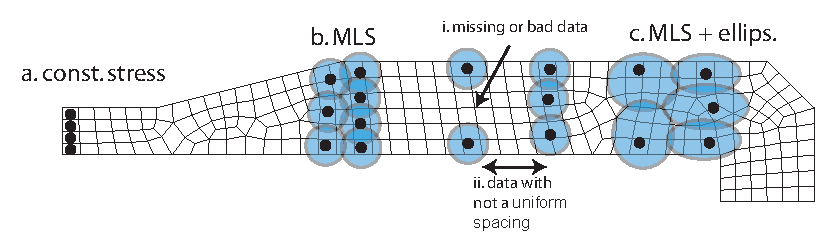
\includegraphics[width=0.9\textwidth]{examplemesh.pdf}
    \caption{An example mesh showing different approaches to find the measured stress vector. \textbf{a.} constant stress assignment to quadrature points reqiures measured data inside each and every finite element of the body (or the mesh should adjusted to be such.), \textbf{b.} MLS method using spheres with constant radii, \textbf{c.} MLS method using ellipsoids with various sizes. }
    \label{figMLS}
\end{figure}


$\mathbf{\sigma_c(x)}$ stands for the interpolated value of measured stress at any position $\mathbf{x}$. We want to find the values of stresses at the quadrature point locations. $\mathbf{\sigma_c}$ refers to the measured stress at the diffraction measurement location $\mathbf{x_c}$. 


MLS method suggests the use of interpolation function, $\mathbf{p}(\mathbf{x})$, with coefficients of $\mathbf{a(x)}$. The variable of interest, in our case it is the interpolated measured stress, $\mathbf{\sigma_c(x)}$, can be calculated at any position if we know the coefficients, $\mathbf{a(x)}$, of the polynomial bases, $\mathbf{p}(\mathbf{x})$. Eq. \eqref{eqMLS} performs this interpolation;

\begin{equation}
\sigma_c(\mathbf{x})\,= \, \mathbf{p}^T(\mathbf{x}) \,\cdot\,\mathbf{a}(\mathbf{x})
\label{eqMLS}
\end{equation}

where $\mathbf{p}(\mathbf{x})$ is the monomial with a linear basis. 
\begin{equation}
\mathbf{p}^T(\mathbf{x})\,= \, [1\; x\; y\; z]
\end{equation}

and $\mathbf{a}(\mathbf{x})$ is the coefficients of that monomial. The square norm of the residual (This residual should not be confused with the residual that is minimized in a weak sense over the finite element mesh and, also with the residual stresses.) becomes as shown in eq. \eqref{eqLSQ} in which $w$ is the weight at location $x$. Summation $\sum_c$ indicates sum over the diffraction measurements. $ndv$ indicates number of diffraction measurements.
\begin{equation}
J\,= \, \sum_c^{ndv} \,w(\mathbf{x}-\mathbf{x_{c}})\,[\mathbf{p}^T(\mathbf{x_c}) \,\cdot\,\mathbf{a}(\mathbf{x_c}) \,-\, \mathbf{\sigma_c}]^2
\label{eqLSQ}
\end{equation}

We want the coefficients that minimize the difference between the measured and interpolated values at the position of measurement, residual. The polynomial coefficients $\mathbf{a}(\mathbf{x}) $ that minimize $J$ is shown in eq. \eqref{eqamin}.
\begin{equation}
\mathbf{a}(\mathbf{x}) \,=\, \mathbf{Y(\mathbf{x})^{-1}} \, \mathbf{Z(\mathbf{x})} \, \mathbf{\sigma_c}
\label{eqamin}
\end{equation}

where
\begin{equation}
\mathbf{Y(\mathbf{x})} \,=\, \sum_{c=1}^{ndv} \, w_c(\mathbf{x}-\mathbf{x_{c}})\, \mathbf{p}^T(\mathbf{x_c})\mathbf{p}(\mathbf{x_c})
\end{equation}

\begin{equation}
\mathbf{Z(\mathbf{x})} \,=\, 
\left[{ \begin{array}{cccccc}
		w_1(\mathbf{x}-\mathbf{x_{1}})\,\mathbf{p(x_1)} & w_2(\mathbf{x}-\mathbf{x_{2}})\,\mathbf{p(x_2)} & \cdots & w_{ndv}(\mathbf{x}-\mathbf{x_{ndv}})\,\mathbf{p(x_{ndv}}) \\
\end{array}} \right]
\end{equation}
 
\begin{equation}
\mathbf{\sigma_c^T} \,=\, \left[{ \begin{array}{cccccc}
		\mathbf{\sigma}_1 & \mathbf{\sigma}_2 & \cdots & \mathbf{\sigma}_{ndv} \\
\end{array}} \right]
\end{equation} 
 
The method is called moving least squares because of the dependence of weight on the position $\mathbf{x}$. This way local character of the measurement is preserved better compared to weighted least square or least square methods. The quartic splines are used as weighting functions.


\begin{equation}
w(q) \,=\,  \left \{ \begin{array}{ll}
					1-6q^2+8q^3-3q^4 & \mbox{if $q < 1$} \\
					0 & \mbox{otherwise}
					\end{array}
					 \right.
\label{eqspline}					 
\end{equation}   

\begin{equation}
q\,=\,  \dfrac{\left\|\mathbf{x}-\mathbf{x_c}\right\| }{\rho}
\end{equation}

$\rho$ is the radius of the diffraction volume for a sphere diffraction volume, fig. \ref{figMLS}. Further details of the method can be found in the ref. \cite{Belytschko96}.



\subsection{MLS with ellipsoids}
The use of spheres with constant radii may cause loss of information. When spheres are used instead of ellipsoids, the user must choose a very large radius to cover the whole disk hence this may cause more information to be lost. Therefore ellipsoids with varying stretch ratios and orientations are constructed around the diffraction volumes from the given diffraction volume coordinates. 

\begin{figure}[!ht]
    \centering
            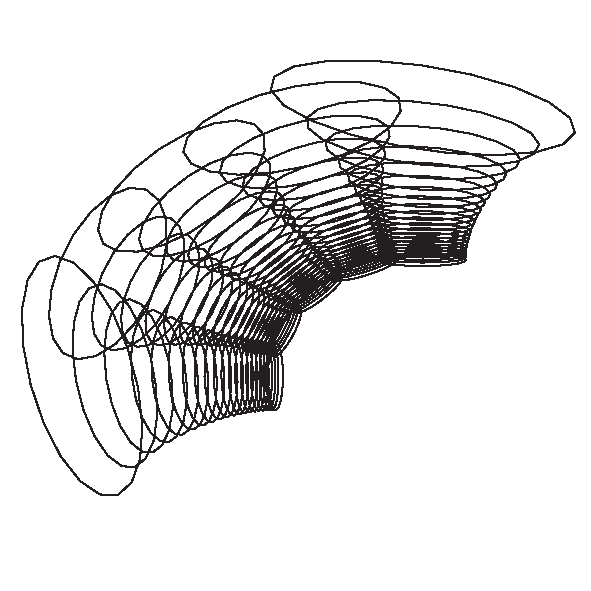
\includegraphics[width=0.5\textwidth]{2Dellipses.pdf}
    \caption{The ellipses that are constructed for a 2D example of a shrink-fit disk problem.}
    \label{2Del}
\end{figure}

Fig. \ref{2Del} shows the ellipses that are constructed for a 2D example of a shrink-fit disk problem using the diffraction volume position coordinates.  

\begin{figure}[!ht]
    \centering
            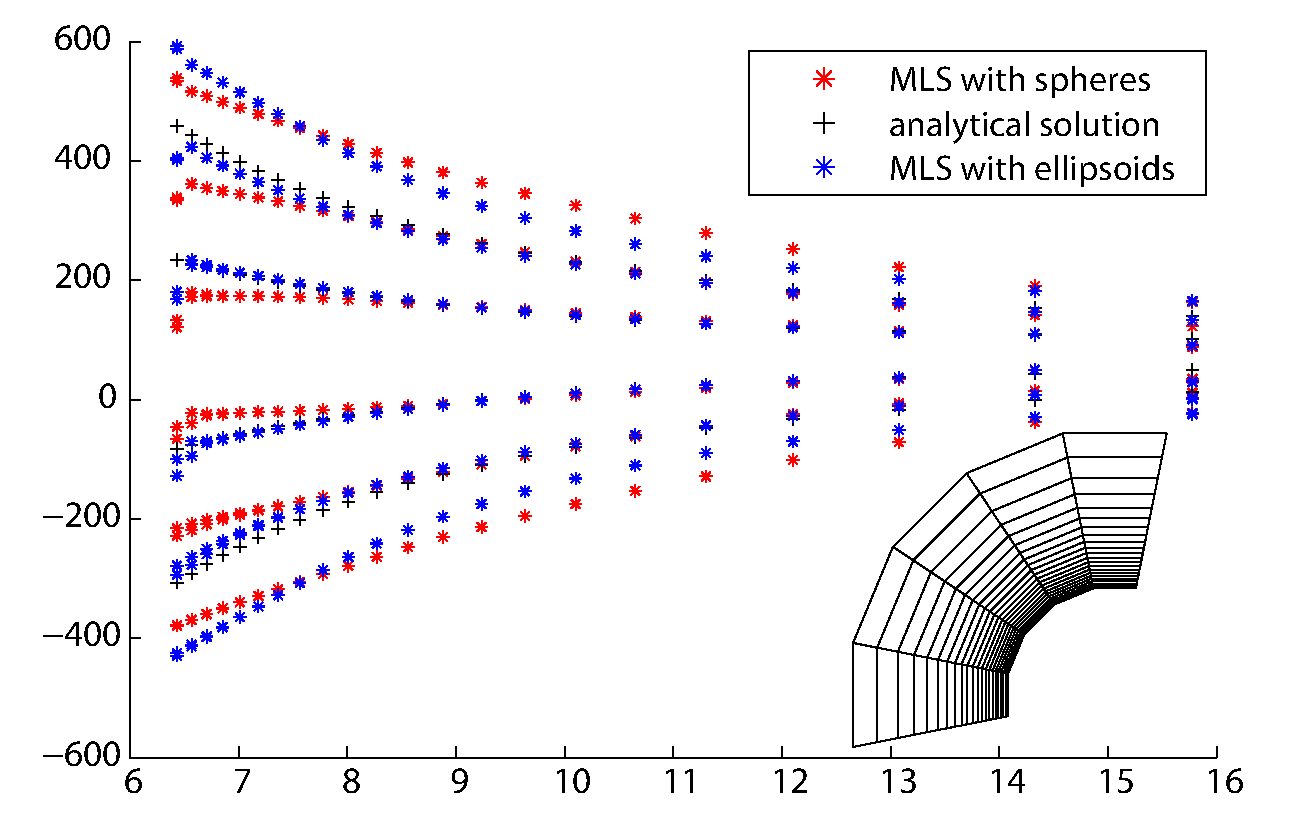
\includegraphics[width=0.7\textwidth]{sphvsel.pdf}
    \caption{$\Sigma^{xx}$ obtained using the analytical solution for the stress at the diffraction data points using spheres vs. ellipsoids and the expected analytical solution. Smallest possible sizes both for the spheres and the ellipsoids are used for comparison.}
    \label{sphvsel}
\end{figure}

The MLS method used for the ellipsoids is the same, only the way that the variable $q$ in eq. \eqref{eqspline} is computed differently for the ellipsoids than the spheres. First, the paramateric equations for the ellipsoids and their orientation are determined. Second, the position under interest is transformed into reference frame of the ellipsoid. Third, the position coordinates of the point (the point at which the weight $w(q)$ is desired - i.e. quadrature points.) is inserted to the equation of the ellipsoid to find the function value of that point. That point would have a function value of unity at the surface of an ellipsoid. Therefore, finally, unity minus the function value at that point is used as the variable $q$ in eq. \eqref{eqspline} for ellipsoids.

The user may need to rescale the size of the ellipsoids since it may not cover a quadrature point in the mesh. Therefore a scaling constant, $\kappa$, is introduced to adjust the size of the ellipsoids.

Fig. \ref{sphvsel}, shows the results obtained using the analytical solution for the stress at the diffraction data points. The use of spheres vs. ellipsoids in conjunction with the MLS method are shown and compared the expected analytical solution at the nodes of the finite element mesh. The use of spheres with constant radii causes loss of information especially at the locations where the diffraction data points tightly spaced as expected. The solution with the ellipsoids gets closer to the expected behavior (analytical solution) in comparison to the results obtained by the use of spheres.


 
%\subsection{special treatment of the boundaries}
%MLS method is used to interpolate the stresses at the quad point locations with least amount of data loss. Any point of interest in the domain, the point must lie inside the ellipsoids (or spheres) of at least 6 number of diffraction data points. This becomes a problem when the point is close to an edge or boundary. Therefore the diffraction data that are nearest to the edges are symmetrically reflected to the other side of the boundary to be able to do the interpolation.

%\begin{figure}
%    \centering
%            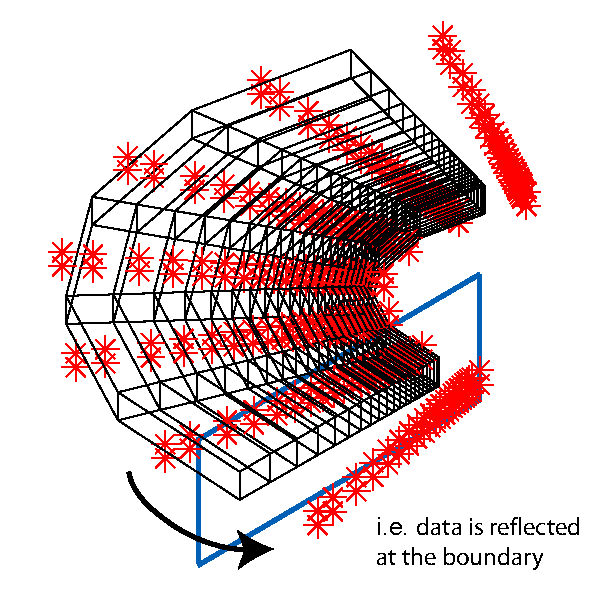
\includegraphics[width=0.7\textwidth]{meshandDVdata.pdf}
%    \caption{An example assignment of diffraction data to the points that lie outside the domain but symmetric with respect to the boundary.}
%    \label{meshandDVdata}
%\end{figure}
%
%Practically speaking, the user must copy the diffraction data that are closest to the boundaries to the other side of the boundary without changing its content. Fig. \ref{meshandDVdata} shows an example assignment of diffraction data to the points that lie outside the domain but symmetric with respect to the boundary.
 




\pagebreak

\appendix

\section{element library}

\subsection{8-node brick element}
Figure \ref{fig1} shows the node numbering used for the volume and surfaces of 8 node brick elements. The order of the nodes of a face of an element must be defined using the nodal ordering\footnote{Nodal ordering of a face of an element must be such that the surface normal of an element must point outward direction.} shown in fig. \ref{fig1}.



\begin{figure}[!ht]
    \centering
            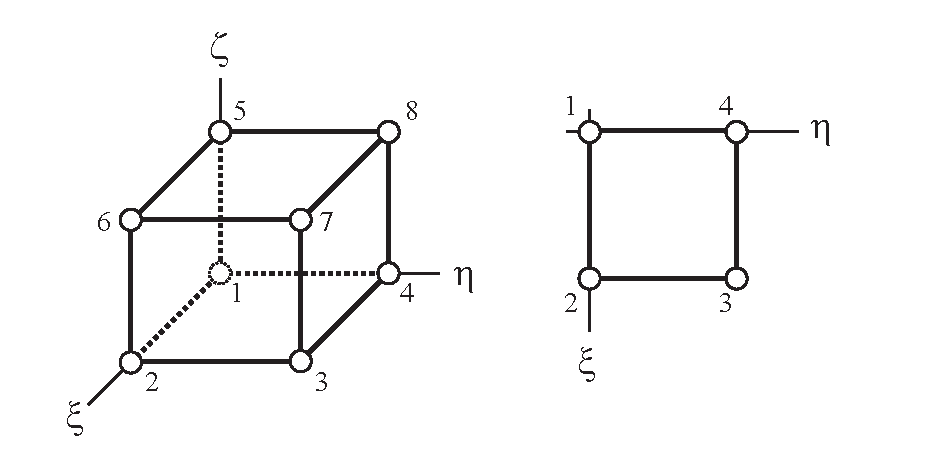
\includegraphics[width=0.8\textwidth]{8nodebrick.pdf}
    \caption{Node numbering of the volume and the surfaces of an 8 node brick element.}
    \label{fig1}
\end{figure}


The shape functions of 8 node brick elements are given as below. Note, the natural coordinates ($\xi$, $\eta$, $\zeta$) range from 0 to +1.  
\begin{eqnarray}
N_1 \;=\; (1-\xi)\, (1-\eta)\, (1-\zeta) \\
N_2 \;=\; \xi\, (1-\eta)\, (1-\zeta) \\
N_3 \;=\; \xi\, \eta\, (1-\zeta) \\
N_4 \;=\; (1-\xi)\, \eta\, (1-\zeta) \\
N_5 \;=\; (1-\xi)\, (1-\eta)\, \zeta \\
N_6 \;=\; \xi\, (1-\eta)\, \zeta \\
N_7 \;=\; \xi\, \eta\, \zeta \\
N_8 \;=\; (1-\xi)\, \eta\, \zeta
\end{eqnarray}


 
%\begin{itemize}
%\item face 1: $\xi$ = 0, 1-5-8-4
%\item face 2: $\xi$ = +1, 2-3-7-6
%\item face 3: $\eta$ = 0, 1-2-6-5
%\item face 4: $\eta$ = +1, 3-4-8-7
%\item face 5: $\zeta$ = 0, 1-4-3-2
%\item face 6: $\zeta$ = +1, 5-6-7-8
%\end{itemize}


\subsection{20-node brick element}

\begin{figure}
    \centering
            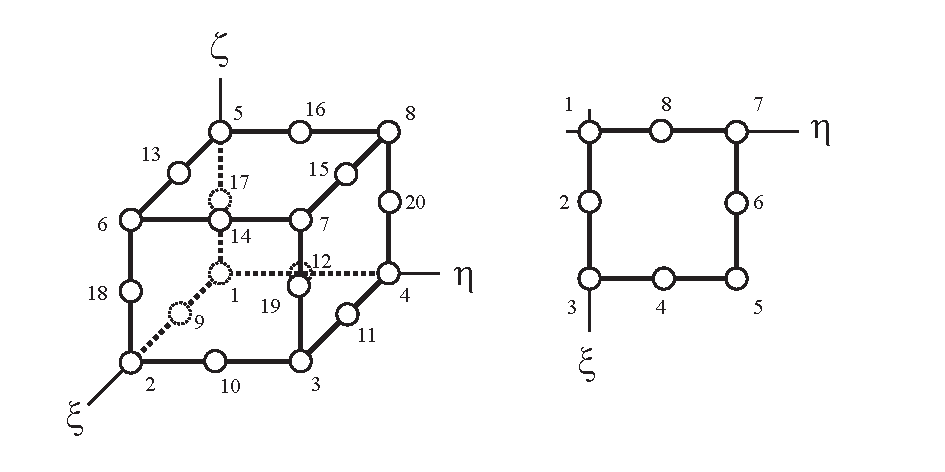
\includegraphics[width=0.7\textwidth]{20nodebrick.pdf}
    \caption{Node numbering of the volume and the surfaces of an 20 node brick element.}
    \label{fig2}
\end{figure}

\begin{eqnarray}
      N_1 \;=\; 2(1-\xi)(1-\eta)(1-\zeta)(0.5-\xi-\eta-\zeta) \\
    	N_2 \;=\;-2\xi(1-\eta)(1-\zeta)(0.5-\xi+\eta+\zeta) \\
    	N_3 \;=\;2\xi\eta(1-\zeta)(\xi+\eta-\zeta-1.5) \\
      N_4 \;=\;-2(1-\xi)\eta(1-\zeta)(0.5+\xi-\eta+\zeta) \\
      N_5 \;=\;-2(1-\xi)(1-\eta)\zeta(0.5+\xi+\eta-\zeta) \\
     	N_6 \;=\;-2\xi(1-\eta)\zeta(1.5-\xi+\eta-\zeta) \\ 
      N_7 \;=\;-2\xi\eta\zeta(2.5-\xi-\eta-\zeta) \\
      N_8 \;=\;-2(1-\xi)\eta\zeta(1.5+\xi-\eta-\zeta) \\
      N_9 \;=\;4\xi(1-\xi)(1-\eta)(1-\zeta) \\
      N_{10} \;=\;4\xi\eta(1-\eta)(1-\zeta) \\
      N_{11} \;=\;4\xi(1-\xi)\eta(1-\zeta) \\
      N_{12} \;=\;4(1-\xi)\eta(1-\eta)(1-\zeta) \\
      N_{13} \;=\;4\xi(1-\xi)(1-\eta)\zeta \\
      N_{14} \;=\;4\xi\eta(1-\eta)\zeta \\
      N_{15} \;=\;4\xi(1-\xi)\eta\zeta     
      N_{16} \;=\;4(1-\xi)\eta(1-\eta)\zeta \\
      N_{17} \;=\;4(1-\xi)(1-\eta)\zeta(1-\zeta) \\
      N_{18} \;=\;4\xi(1-\eta)\zeta(1-\zeta) \\
      N_{19} \;=\;4\xi\eta\zeta(1-\zeta) \\
      N_{20} \;=\;4(1-\xi)\eta\zeta(1-\zeta)
 \end{eqnarray}


\subsection{27-node brick element}
\begin{figure}[ht!]
    \centering
            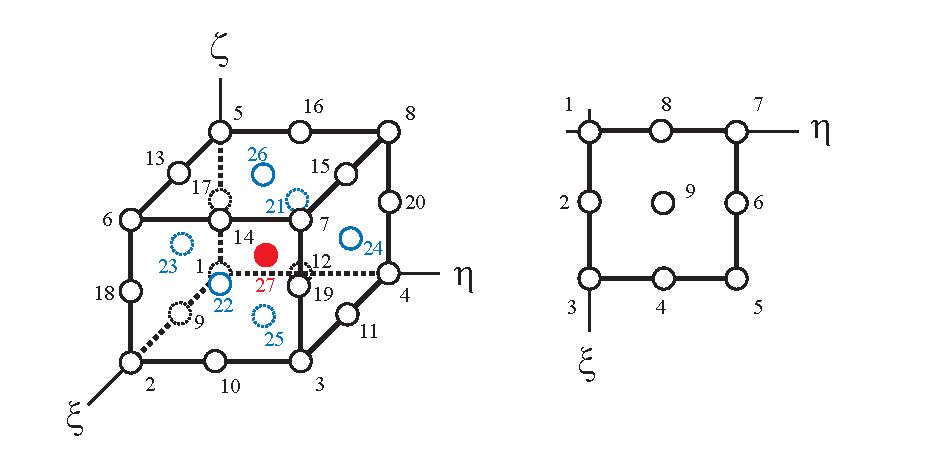
\includegraphics[width=0.7\textwidth]{27nodebrick.pdf}
    \caption{Node numbering of the volume and the surfaces of an 27 node brick element.}
    \label{fig3}
\end{figure}

\begin{eqnarray}   
	N_{1} \;=\; (1-2\xi)(1-\xi)(1-2\eta)(1-\eta)(1-2\zeta)(1-\zeta) \\
	N_{2} \;=\; -(1-2\xi)\xi(1-2\eta)(1-\eta)(1-2\zeta)(1-\zeta) \\
	N_{3} \;=\; (1-2\xi)\xi(1-2\eta)\eta(1-2\zeta)(1-\zeta) \\
	N_{4} \;=\; -(1-2\xi)(1-\xi)(1-2\eta)\eta(1-2\zeta)(1-\zeta) \\
	N_{5} \;=\; -(1-2\xi)(1-\xi)(1-2\eta)(1-\eta)(1-2\zeta)\zeta \\
	N_{6} \;=\; (1-2\xi)\xi(1-2\eta)(1-\eta)(1-2\zeta)\zeta \\
	N_{7} \;=\; -(1-2\xi)\xi(1-2\eta)\eta(1-2\zeta)\zeta \\
	N_{8} \;=\; (1-2\xi)(1-\xi)(1-2\eta)\eta(1-2\zeta)\zeta \\
	N_{9} \;=\; 4\xi(1-\xi)(1-2\eta)(1-\eta)(1-2\zeta)(1-\zeta) \\
	N_{10} \;=\; -4(1-2\xi)\xi\eta(1-\eta)(1-2\zeta)(1-\zeta) \\
	N_{11} \;=\; -4\xi(1-\xi)(1-2\eta)\eta(1-2\zeta)(1-\zeta) \\
	N_{12} \;=\; 4(1-2\xi)(1-\xi)\eta(1-\eta)(1-2\zeta)(1-\zeta) \\
	N_{13} \;=\; -4\xi(1-\xi)(1-2\eta)(1-\eta)(1-2\zeta)\zeta \\
	N_{14} \;=\; 4(1-2\xi)\xi\eta(1-\eta)(1-2\zeta)\zeta \\ 
	N_{15} \;=\; 4\xi(1-\xi)(1-2\eta)\eta(1-2\zeta)\zeta \\
	N_{16} \;=\; -4(1-2\xi)(1-\xi)\eta(1-\eta)(1-2\zeta)\zeta \\
	N_{17} \;=\; 4(1-2\xi)(1-\xi)(1-2\eta)(1-\eta)\zeta(1-\zeta) \\
	N_{18} \;=\; -4(1-2\xi)\xi(1-2\eta)(1-\eta)\zeta(1-\zeta) \\
	N_{19} \;=\; 4(1-2\xi)\xi(1-2\eta)\eta\zeta(1-\zeta) \\
	N_{20} \;=\; -4(1-2\xi)(1-\xi)(1-2\eta)\eta\zeta(1-\zeta) \\
	N_{21} \;=\; 16(1-2\xi)(1-\xi)\eta(1-\eta)\zeta(1-\zeta) \\
	N_{22} \;=\; -16(1-2\xi)\xi\eta(1-\eta)\zeta(1-\zeta) \\
	N_{23} \;=\; -16\xi(1-\xi)(1-2\eta)\eta\zeta(1-\zeta) \\
	N_{24} \;=\; 16\xi(1-\xi)(1-2\eta)(1-\eta)\zeta(1-\zeta) \\
	N_{25} \;=\; 16\xi(1-\xi)\eta(1-\eta)(1-2\zeta)(1-\zeta) \\
 \end{eqnarray}

\begin{eqnarray}   
	N_{26} \;=\; -16\xi(1-\xi)\eta(1-\eta)(1-2\zeta)\zeta \\
	N_{27} \;=\; 64\xi(1-\xi)\eta(1-\eta)\zeta(1-\zeta)
 \end{eqnarray}


\subsection{10-node tetragonal element}

\begin{figure}[ht!]
    \centering
            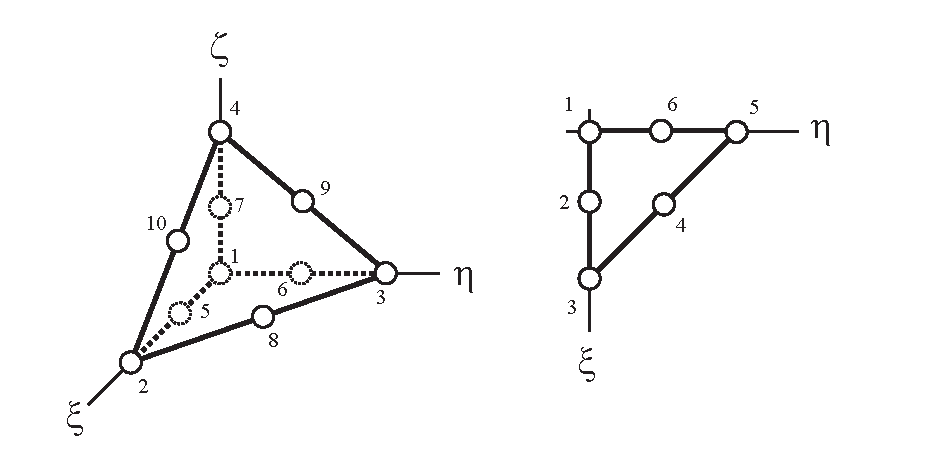
\includegraphics[width=0.4\textwidth]{10nodetet.pdf}
    \caption{Node numbering of the volume and the surfaces of an 10 node tetragonal element.}
    \label{fig4}
\end{figure}

\begin{eqnarray}
   N_{1} \;=\;(1-2\xi-2\eta-2\zeta)(1-\xi-\eta-\zeta) \\
   N_{2} \;=\;(2\xi-1)\xi \\
   N_{3} \;=\;(2\eta-1)\eta \\
   N_{4} \;=\;(2\zeta-1)\zeta \\
   N_{5} \;=\;4\xi(1-\xi-\eta-\zeta) \\
   N_{6} \;=\;4\eta(1-\xi-\eta-\zeta) \\
   N_{7} \;=\;4\zeta(1-\xi-\eta-\zeta) \\
   N_{8} \;=\;4\xi\eta \\
   N_{9} \;=\;4\eta\zeta \\
   N_{10} \;=\;4\xi\zeta \\
\end{eqnarray}



\section{inputs to the code}


The inputs used in the analysis:
\begin{itemize}
\item \textbf{numel}: total number of elements in the mesh
\item \textbf{numnp}: total number of nodes in the mesh
\item \textbf{meltyp}: element type (8: 8 node brick, 20: 20 node brick, 27: 27 node brick, 10: 10 node tetrahedra)
\item \textbf{x,y,z}: node coordinates
\item \textbf{np}: element connectivity matrix
\item \textbf{nps}: node numbers of each traction free surface (IMPORTANT: Node ordering must be such that counter-clockwise rotation must give the surface normal pointing OUTWARDS!)
\item \textbf{npsyms}: node numbers of each symmetric surface (node ordering is important for the same reason as the traction free surfaces!)
\item $\lambda$ : penalty factor for equilibrium constraint
\item $\alpha$ : penalty factor for symmetry surface constraint
\item $\beta$ : penalty factor for traction free surface constraint
\item $\kappa$ : scaling constant to adjust the size of the ellipsoids
%\item \textbf{rho}: magnitude of radius that the diffraction volume covers (The magnitude must be selected such that all the quadrature points in the mesh are in the range of at least one measured diffraction volume.)
\end{itemize}

The inputs for the mesh are given in the file mesh$\_$data.m. The other inputs are declared in the main m-file; Residual$\_$Stress$\_$3d.m.

\section{example: shrink fit disc}

The analysis is applied to a portion of a disk that is shrink fitted to a shaft. The magnitudes of stresses at the quadrature points are found using the analytical solution to the problem. The surface constraints are shown in fig. \ref{fig5}.


\begin{figure}[ht!]
    \centering
            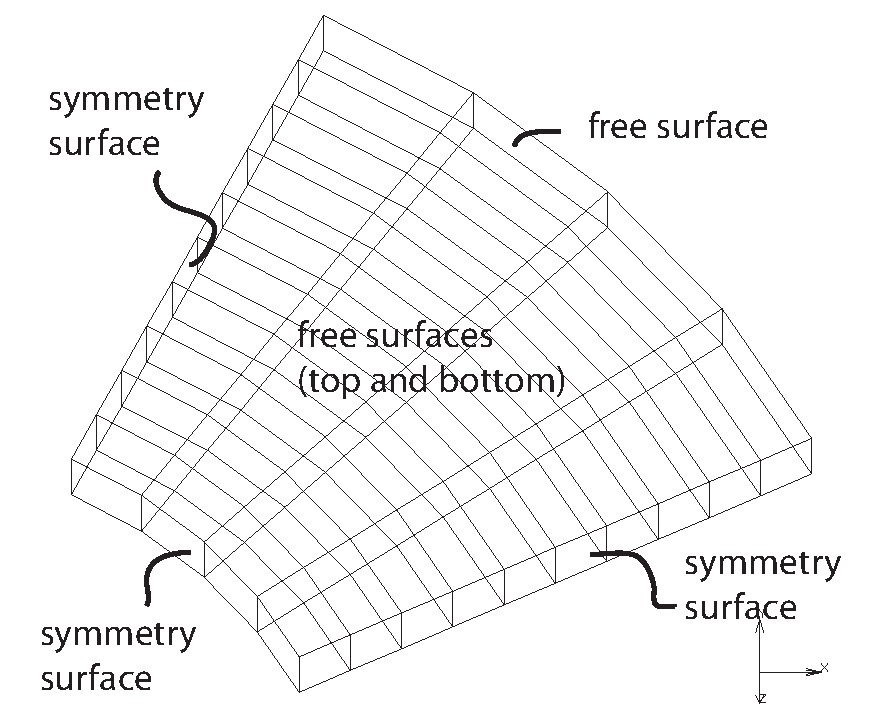
\includegraphics[width=0.3\textwidth]{discbcs.pdf}
    \caption{Surface constraints of the shrink fit disc problem.}
    \label{fig5}
\end{figure}


The symmetry constraints allow us to study only a portion of disc. The stress distribution is obtained for the surface constraints together with the equilibrium constraint over the whole disc, fig. \ref{fig6}.


\begin{figure}[ht!]
    \centering
            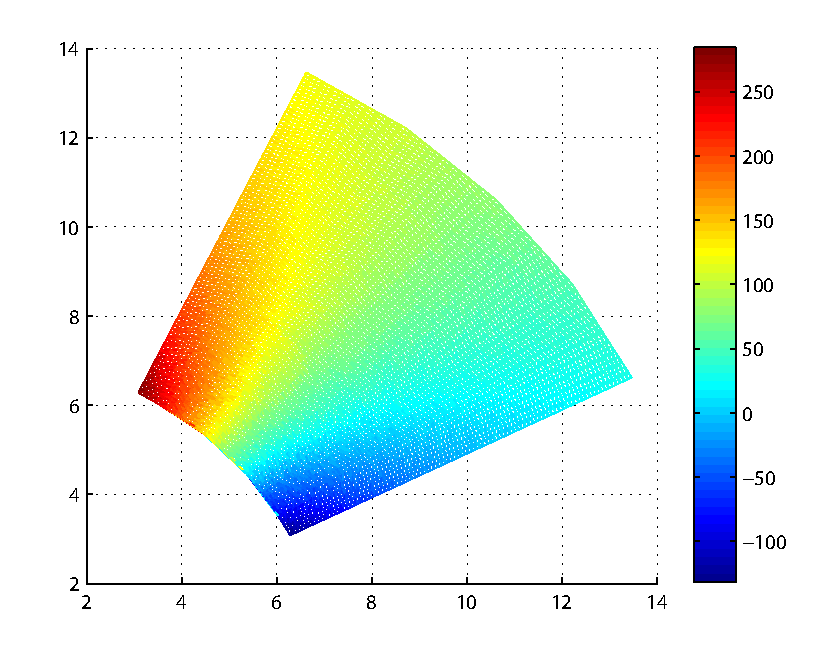
\includegraphics[width=0.4\textwidth]{discbotsigxx.pdf}
    \caption{Results of the 3d analysis: $\Sigma(x)^{xx}$ at the bottom surface of the disc.}
    \label{fig6}
\end{figure}





\small
\begin{thebibliography}{99}
\setlength{\itemsep}{-0.5mm}
\bibitem{Belytschko96} Beissel, S., Belytschko, T., 1996. Nodal integration of the element-free Galerkin method. Comp. Met. in App. Mech. and Eng. 139, 49-74.
%
\end{thebibliography}



\end{document}